\begin{figure}[H]
    \centering
    \begin{tikzpicture}
        \pgfplotsset{
            width=0.4\textwidth,
            height=0.5\textheight
        }
        \begin{axis}
            [
                xbar,
                legend style={at={(0.5,-0.1)}, anchor=north,legend columns=-1},
                bar width = 5pt,
                xlabel= DEC (Joules),
                xmin=0,xmax=1100,
                symbolic y coords = {
                    IPG, 
                    LHM, 
                    SCAP, 
                    SCAPI, 
                    {Clamp (W)}, 
                    {Plug (W)},
                    RAPL,
                    {Clamp (L)},
                    {Plug (L)}},
            ]
            \addplot coordinates { 
                (524.49,IPG)
                (517.275,LHM)
                (524.18,SCAP)
                (659.47,SCAPI)
                (677.93,{Clamp (W)})
                (758.63,{Plug (W)})
                (325.89,RAPL)
                (1058,{Clamp (L)})
                (836.47,{Plug (L)})
                };
            \addplot coordinates { 
                (415.05,IPG)
                (426.03,LHM)
                (451.05,SCAP)
                (565.55,SCAPI)
                (327.41,{Clamp (W)})
                (448.67,{Plug (W)})
                (557.63,RAPL)
                (651,{Clamp (L)})
                (752.80,{Plug (L)})
                };
            \legend{FR, MB}
            \end{axis}
        \end{tikzpicture}
    \caption{The average DEC for DUT 1, where both benchmarks are compiled on oneAPI} \label{fig:dut-1-compare-mi}
\end{figure}
